%=====================================================================
% Modelo de datos · Diagrama entidad-relación
%   Las figuras de er/salida se generan con er/generar.py a partir de
%   er/esquema.json (que exporta bd/generar_tablas.ps1) y de
%   er/diagramas.py. No se editan a mano.
%=====================================================================
\subsection*{Diagrama entidad-relación}
\addcontentsline{toc}{subsection}{Diagrama entidad-relación}

Los diagramas de esta subsección son el modelo actualizado, en la misma notación de Chen del diagrama original. No se dibujaron a mano: \at{er/generar.py} los construye a partir del esquema que exporta \at{bd/generar\_tablas.ps1}, de modo que muestran exactamente las tablas, columnas y llaves foráneas del script \at{bd/crear\_tablas.sql}. Cada uno existe además como archivo \at{.drawio}, editable en app.diagrams.net, en \at{er/salida}. Las figuras son vectoriales: los nombres de los atributos se leen ampliando el PDF, o en los \at{.svg} de la misma carpeta.

Un solo dibujo con \bdNumTablas{} entidades y \bdNumColumnas{} atributos no se podría leer, así que el modelo se presenta en una vista general, con todas las entidades y relaciones pero sin atributos, y en un diagrama por área con todos sus atributos. En cada diagrama de área aparecen también, sin atributos, las entidades de otras áreas que sus relaciones tocan; sus atributos están en el diagrama de su propia área.

\subsubsection*{Cómo se leen}
\addcontentsline{toc}{subsubsection}{Cómo se leen}

\begin{reglas}
  \item \textbf{Entidades.} Cada tabla es una entidad, dibujada como rectángulo. Las que se identifican por la llave de otra ---débiles, asociativas y dependientes, según la tabla de identificación de entidades--- llevan doble marco.
  \item \textbf{Relaciones.} Cada llave foránea es una relación, dibujada como rombo con un verbo. El rombo es doble cuando la relación es identificadora, es decir, cuando las columnas de la llave foránea forman parte de la llave primaria de la hija.
  \item \textbf{Atributos.} Son óvalos unidos a su entidad. Los de la llave primaria van subrayados; en una entidad débil, el subrayado marca su discriminador, como \at{numero\_jugada} en \textit{Jugada}. Los de línea punteada son las columnas calculadas. Las columnas de una llave foránea no se dibujan como atributos, porque las representa la relación.
  \item \textbf{Razón.} Sobre cada rombo va la razón (\at{1:N}, \at{N:1} o \at{1:1}), y la flecha apunta al lado 1. Se lee siguiendo la frase del rombo: «\textit{Usuario} abre \textit{Sesion}» es 1:N y «\textit{Reporte} señala a \textit{Usuario}» es N:1.
  \item \textbf{Pares de cardinalidad.} Junto a cada entidad van dos cifras. La de arriba se lee siguiendo la frase del rombo, del sujeto al objeto; la de abajo, al revés. El sujeto lleva arriba siempre 1.
  \item \textbf{Participación.} La doble línea marca participación total: toda fila de esa entidad participa en la relación. Del lado de la hija corresponde a una llave foránea obligatoria; del lado del padre, a una regla de negocio, como las estadísticas de cada modo y los objetos iniciales que el alta crea para todo usuario (\mbox{CU-02} \mbox{RN-06}). La línea simple marca participación parcial. En el archivo \at{.drawio} la doble línea oculta la flecha, porque draw.io no dibuja las dos cosas a la vez.
  \item \textbf{Papeles.} Cuando una entidad participa dos veces en relaciones con la misma otra entidad, cada línea lleva su papel en cursiva: el emisor y el destinatario de una invitación, el reportante y el reportado de un reporte.
  \item \textbf{Relación recursiva.} La única relación de una entidad consigo misma, la sanción que sustituye a otra (\mbox{CU-44} \mbox{RN-09}), se dibuja con dos líneas paralelas hacia \textit{Sancion}, una por papel.
\end{reglas}

Hay restricciones que ninguna notación de cardinalidad expresa y que el esquema garantiza de otro modo. Que una partida tenga uno, dos o cuatro participantes según su tipo y su modo lo garantiza la transacción que la crea (\mbox{CU-17} \mbox{RN-10}); que un usuario tenga una sola participación sin terminar (\mbox{D-11}), el índice único filtrado de \textit{Participacion}.

%---------------------------------------------------------------------
% Vista general
%---------------------------------------------------------------------
\clearpage
\subsubsection*{Vista general}
\addcontentsline{toc}{subsubsection}{Vista general}
Las \bdNumTablas{} entidades y sus \bdNumForaneas{} relaciones, sin atributos. \textit{Usuario} queda en el centro porque es la entidad de la que depende casi todo el modelo.
\begin{center}
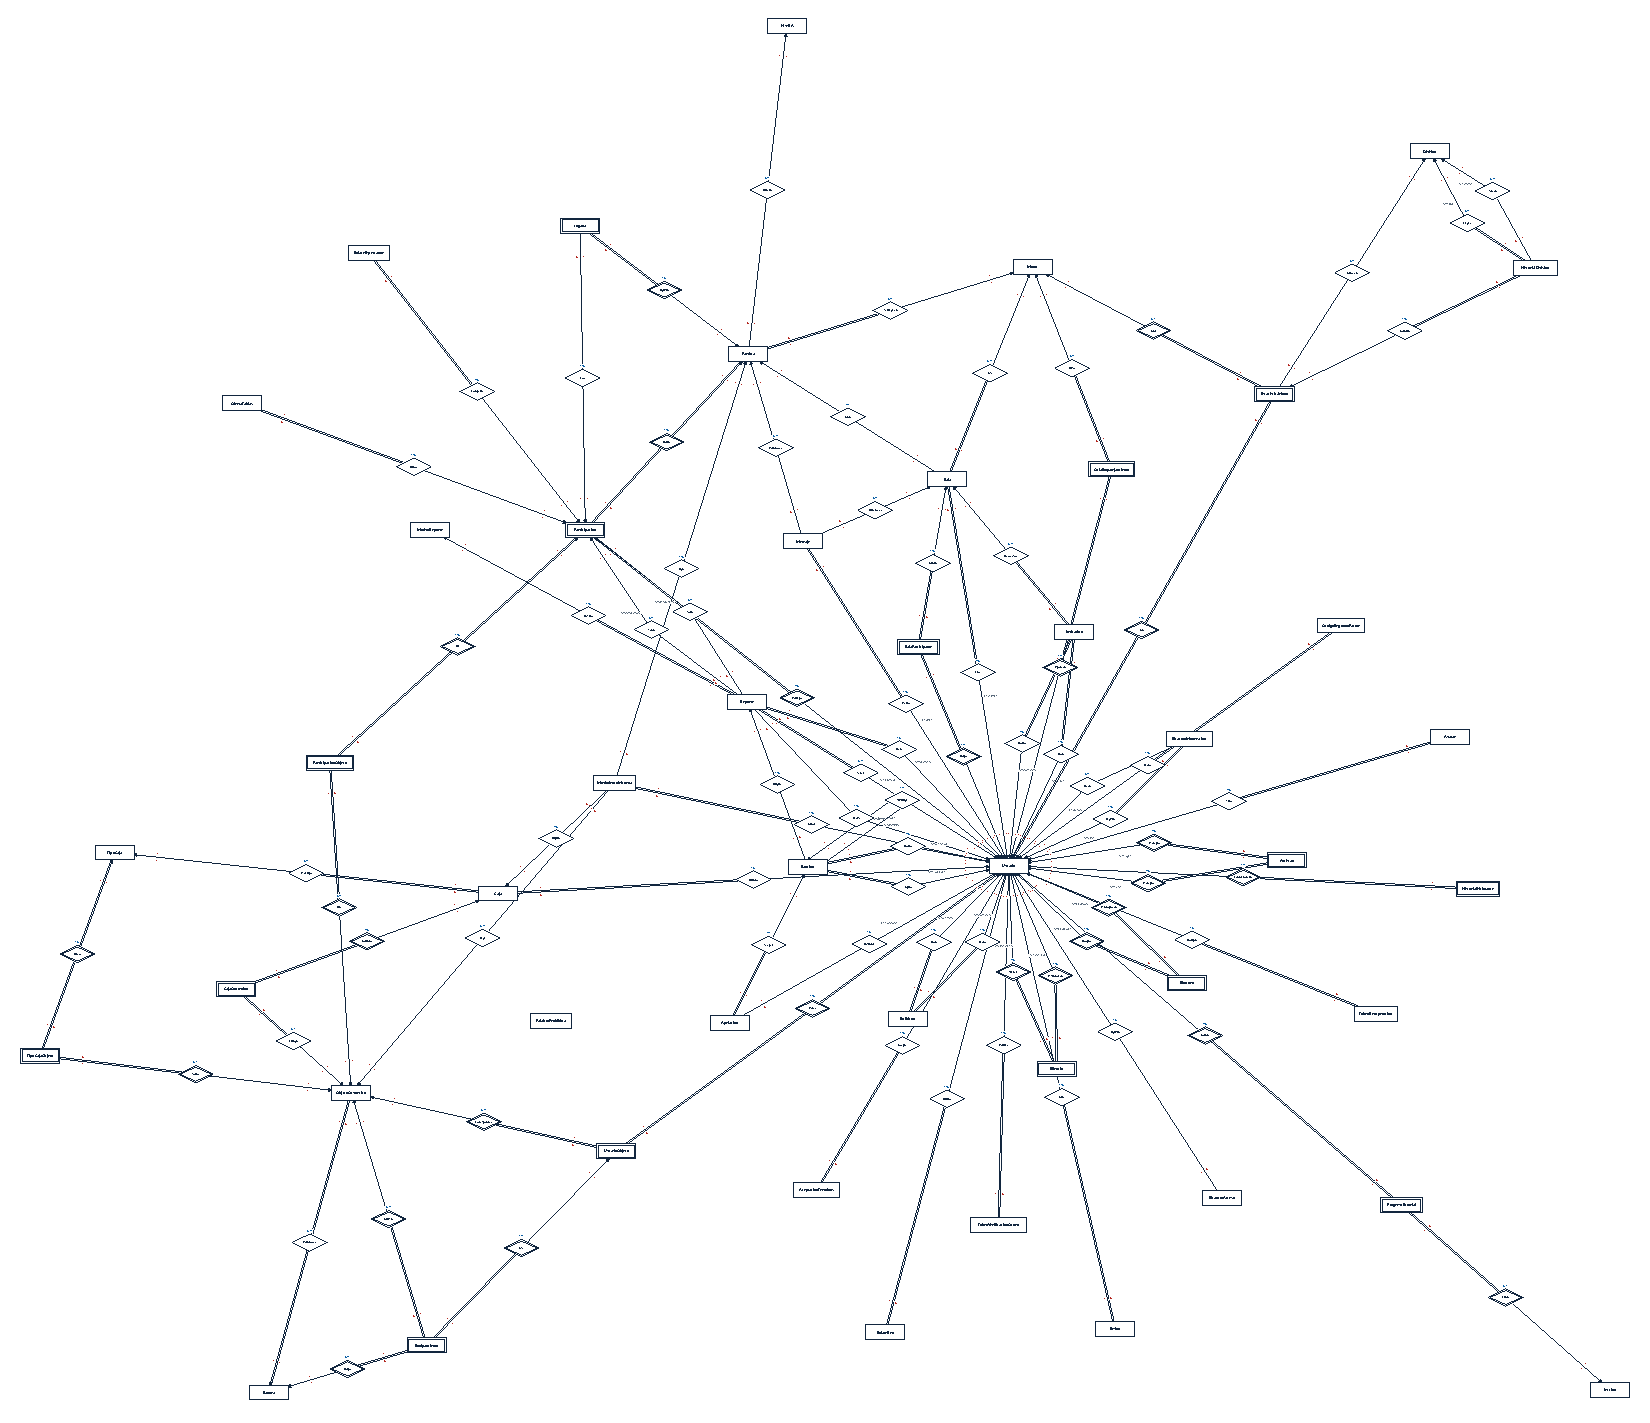
\includegraphics[width=\linewidth,height=0.82\textheight,keepaspectratio]{er/salida/general}
\end{center}

%---------------------------------------------------------------------
% Un diagrama por área, en el orden de las tablas de atributos
%---------------------------------------------------------------------
\begin{landscape}
\subsubsection*{Catálogos precargados}
\addcontentsline{toc}{subsubsection}{Diagrama: catálogos precargados}
Los diez catálogos que se cargan por SQL (\mbox{D-09}). Solo tres se relacionan entre sí: cada objeto pertenece a una ranura y cada tipo de caja sortea objetos con su probabilidad. Ninguno guarda nombres visibles: cada fila tiene un \at{codigo}, la clave de su nombre en los diccionarios de recursos (\mbox{D-21}).
\begin{center}
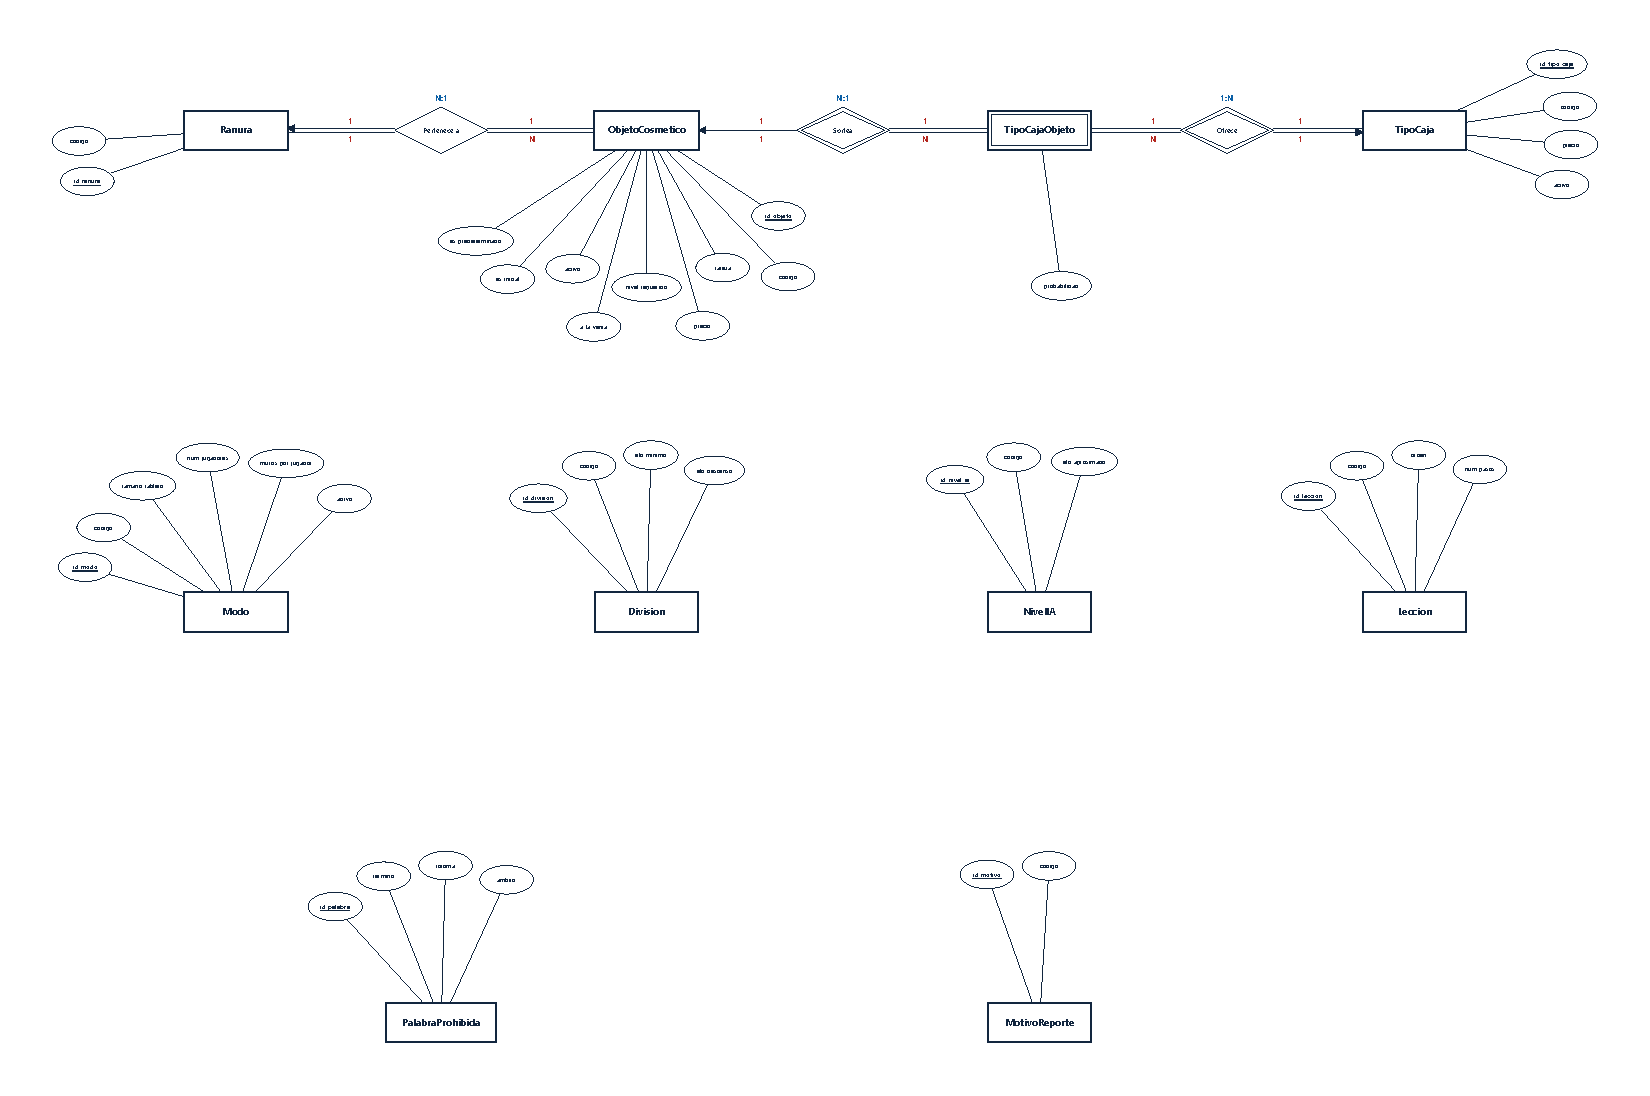
\includegraphics[width=\linewidth,height=0.8\textheight,keepaspectratio]{er/salida/catalogos}
\end{center}
\end{landscape}

\clearpage
\subsubsection*{Cuenta y acceso}
\addcontentsline{toc}{subsubsection}{Diagrama: cuenta y acceso}
\textit{Usuario} con todos sus atributos, y las sesiones, los códigos, los tokens y las aceptaciones de términos que dependen de él.
\begin{center}
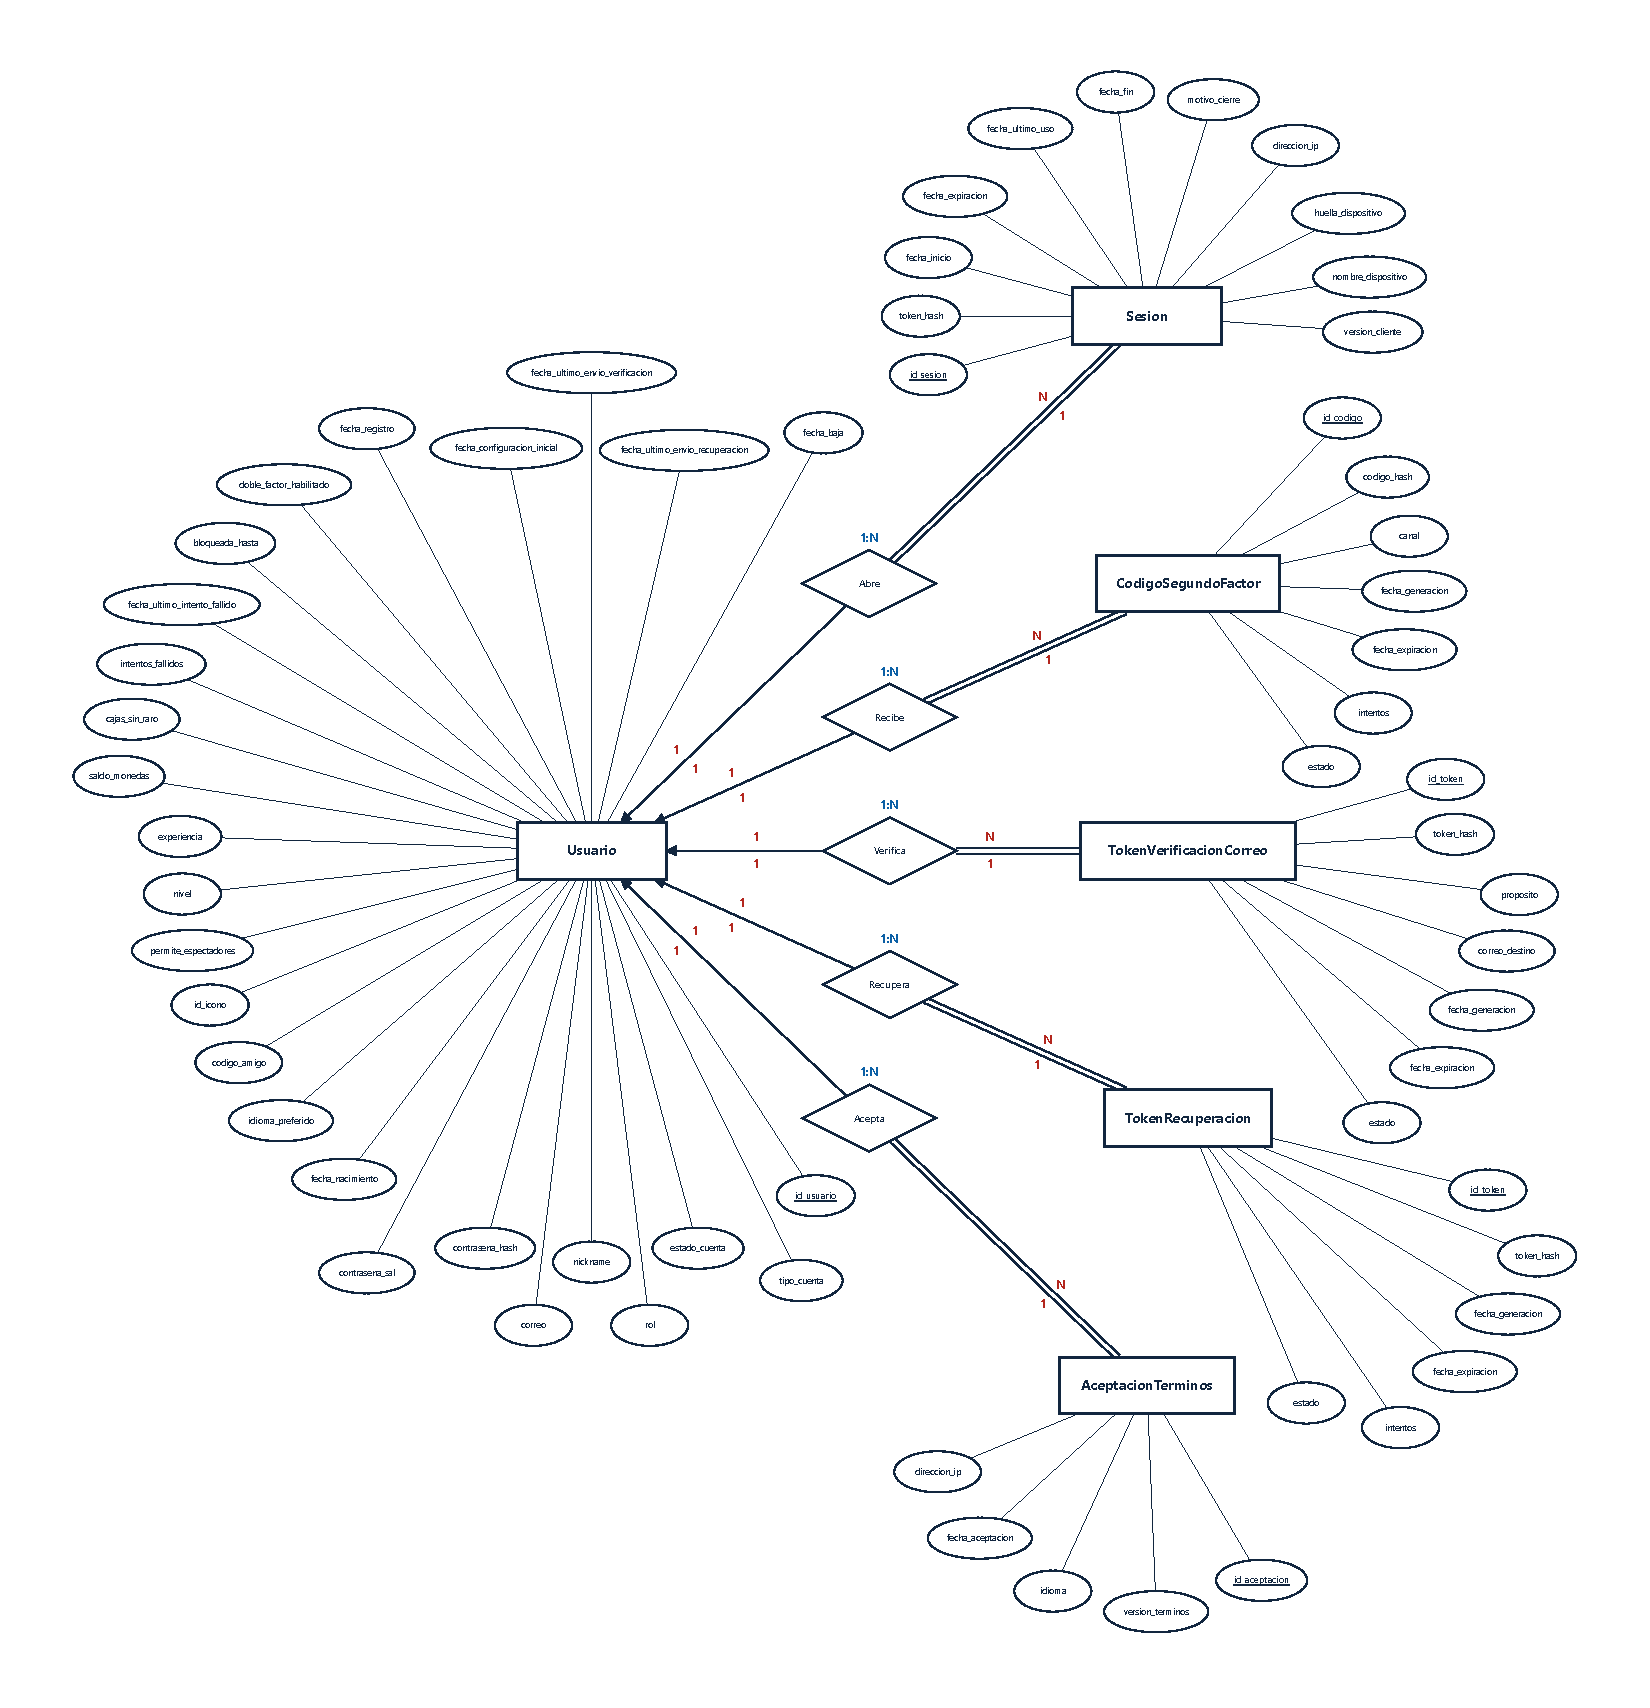
\includegraphics[width=\linewidth,height=0.82\textheight,keepaspectratio]{er/salida/cuenta}
\end{center}

\begin{landscape}
\subsubsection*{Perfil y personalización}
\addcontentsline{toc}{subsubsection}{Diagrama: perfil y personalización}
El perfil público y los objetos cosméticos: lo que el jugador posee (\textit{UsuarioObjeto}) y lo que lleva equipado en cada ranura (\textit{Equipamiento}), que solo puede ser algo que posee.
\begin{center}
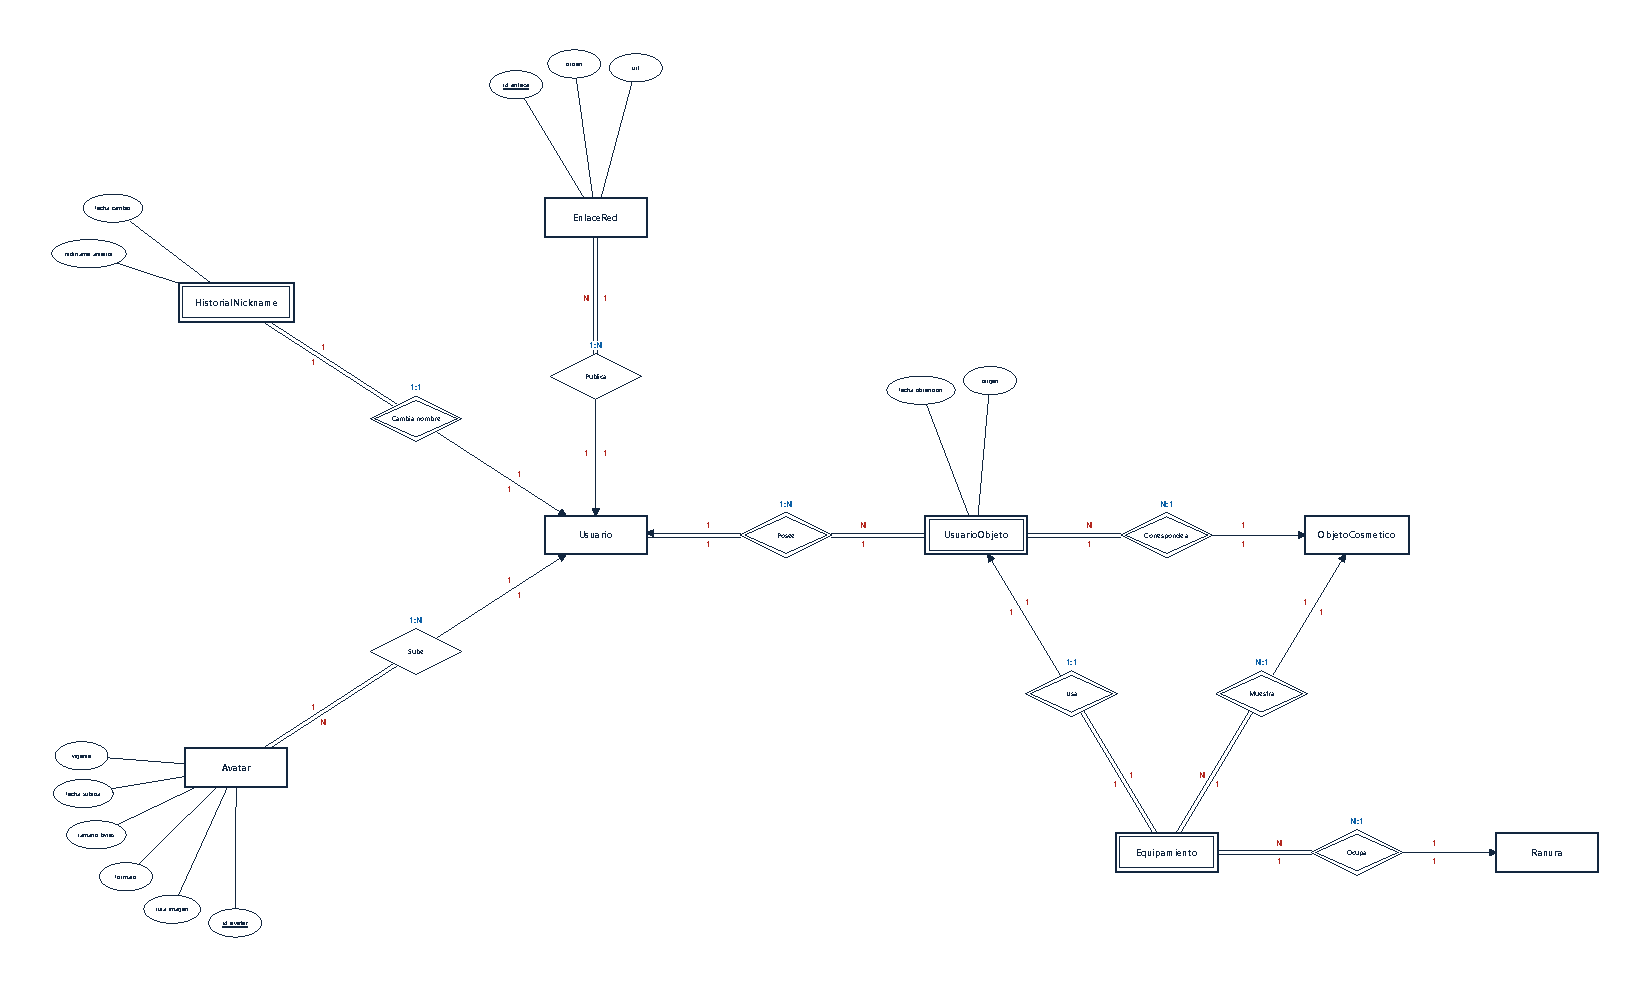
\includegraphics[width=\linewidth,height=0.8\textheight,keepaspectratio]{er/salida/perfil}
\end{center}
\end{landscape}

\begin{landscape}
\subsubsection*{Partida}
\addcontentsline{toc}{subsubsection}{Diagrama: partida}
La partida y la participación de cada jugador, con las jugadas, las ofertas de tablas, los enlaces de espectador y el aspecto fijado al empezar. El ganador no es una relación aparte: es la participación con resultado \at{GANADA}.
\begin{center}
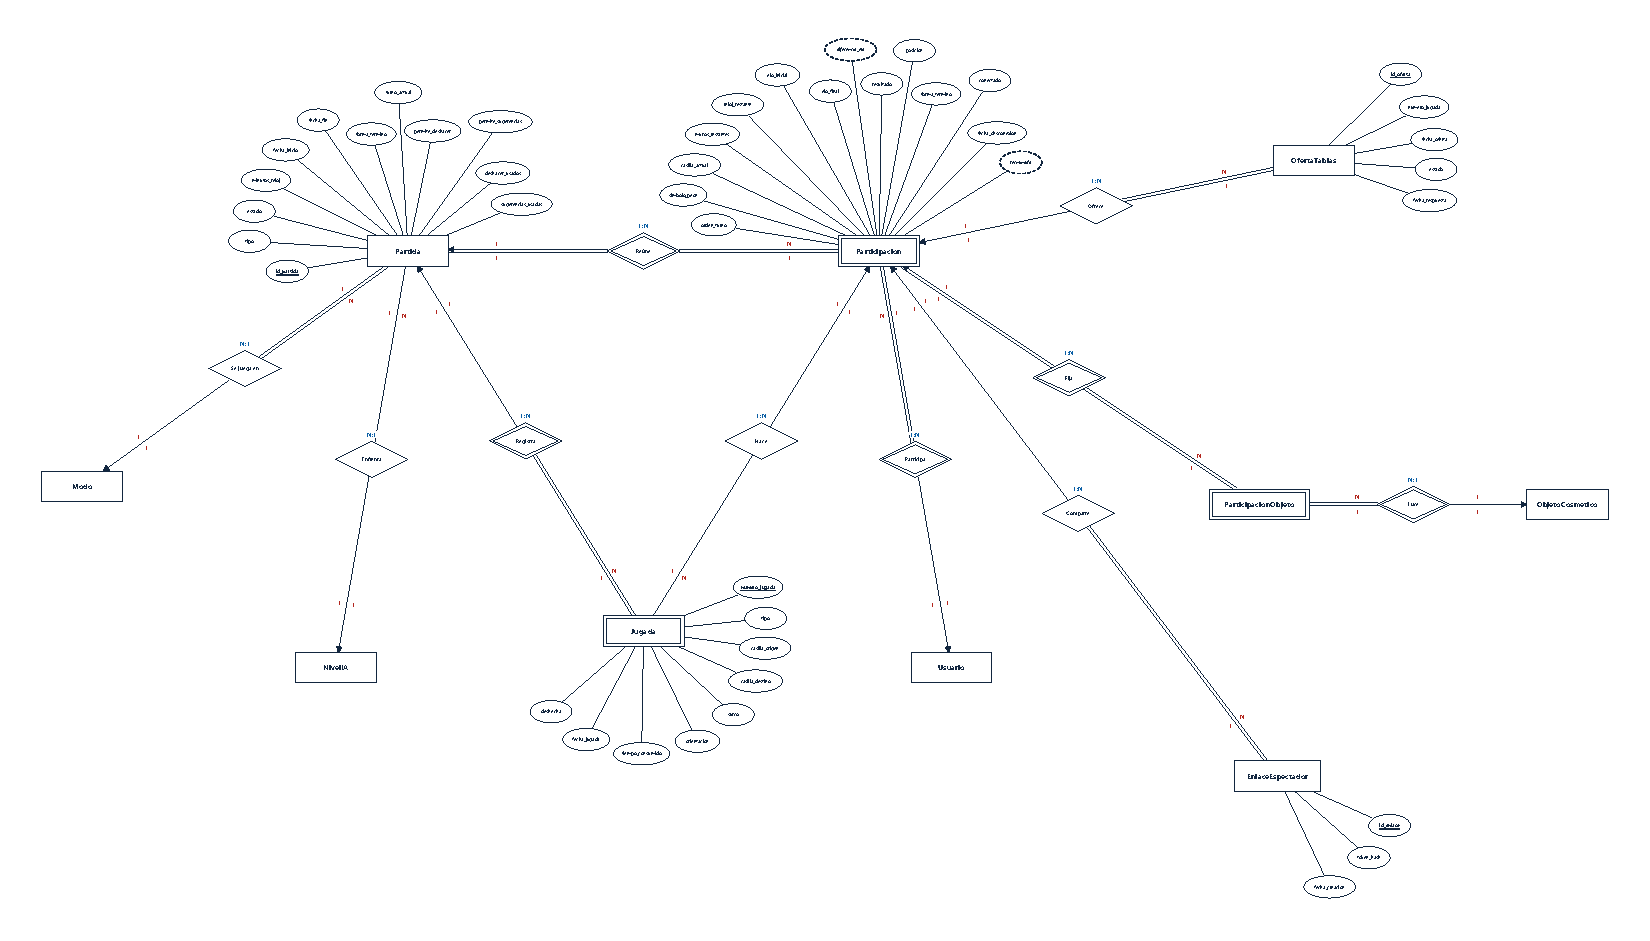
\includegraphics[width=\linewidth,height=0.8\textheight,keepaspectratio]{er/salida/partida}
\end{center}
\end{landscape}

\clearpage
\subsubsection*{Emparejamiento, salas y chat}
\addcontentsline{toc}{subsubsection}{Diagrama: emparejamiento, salas y chat}
La cola clasificatoria, las salas privadas con sus plazas e invitaciones, y los mensajes, que pertenecen a una partida, a una sala o a un canal general.
\begin{center}
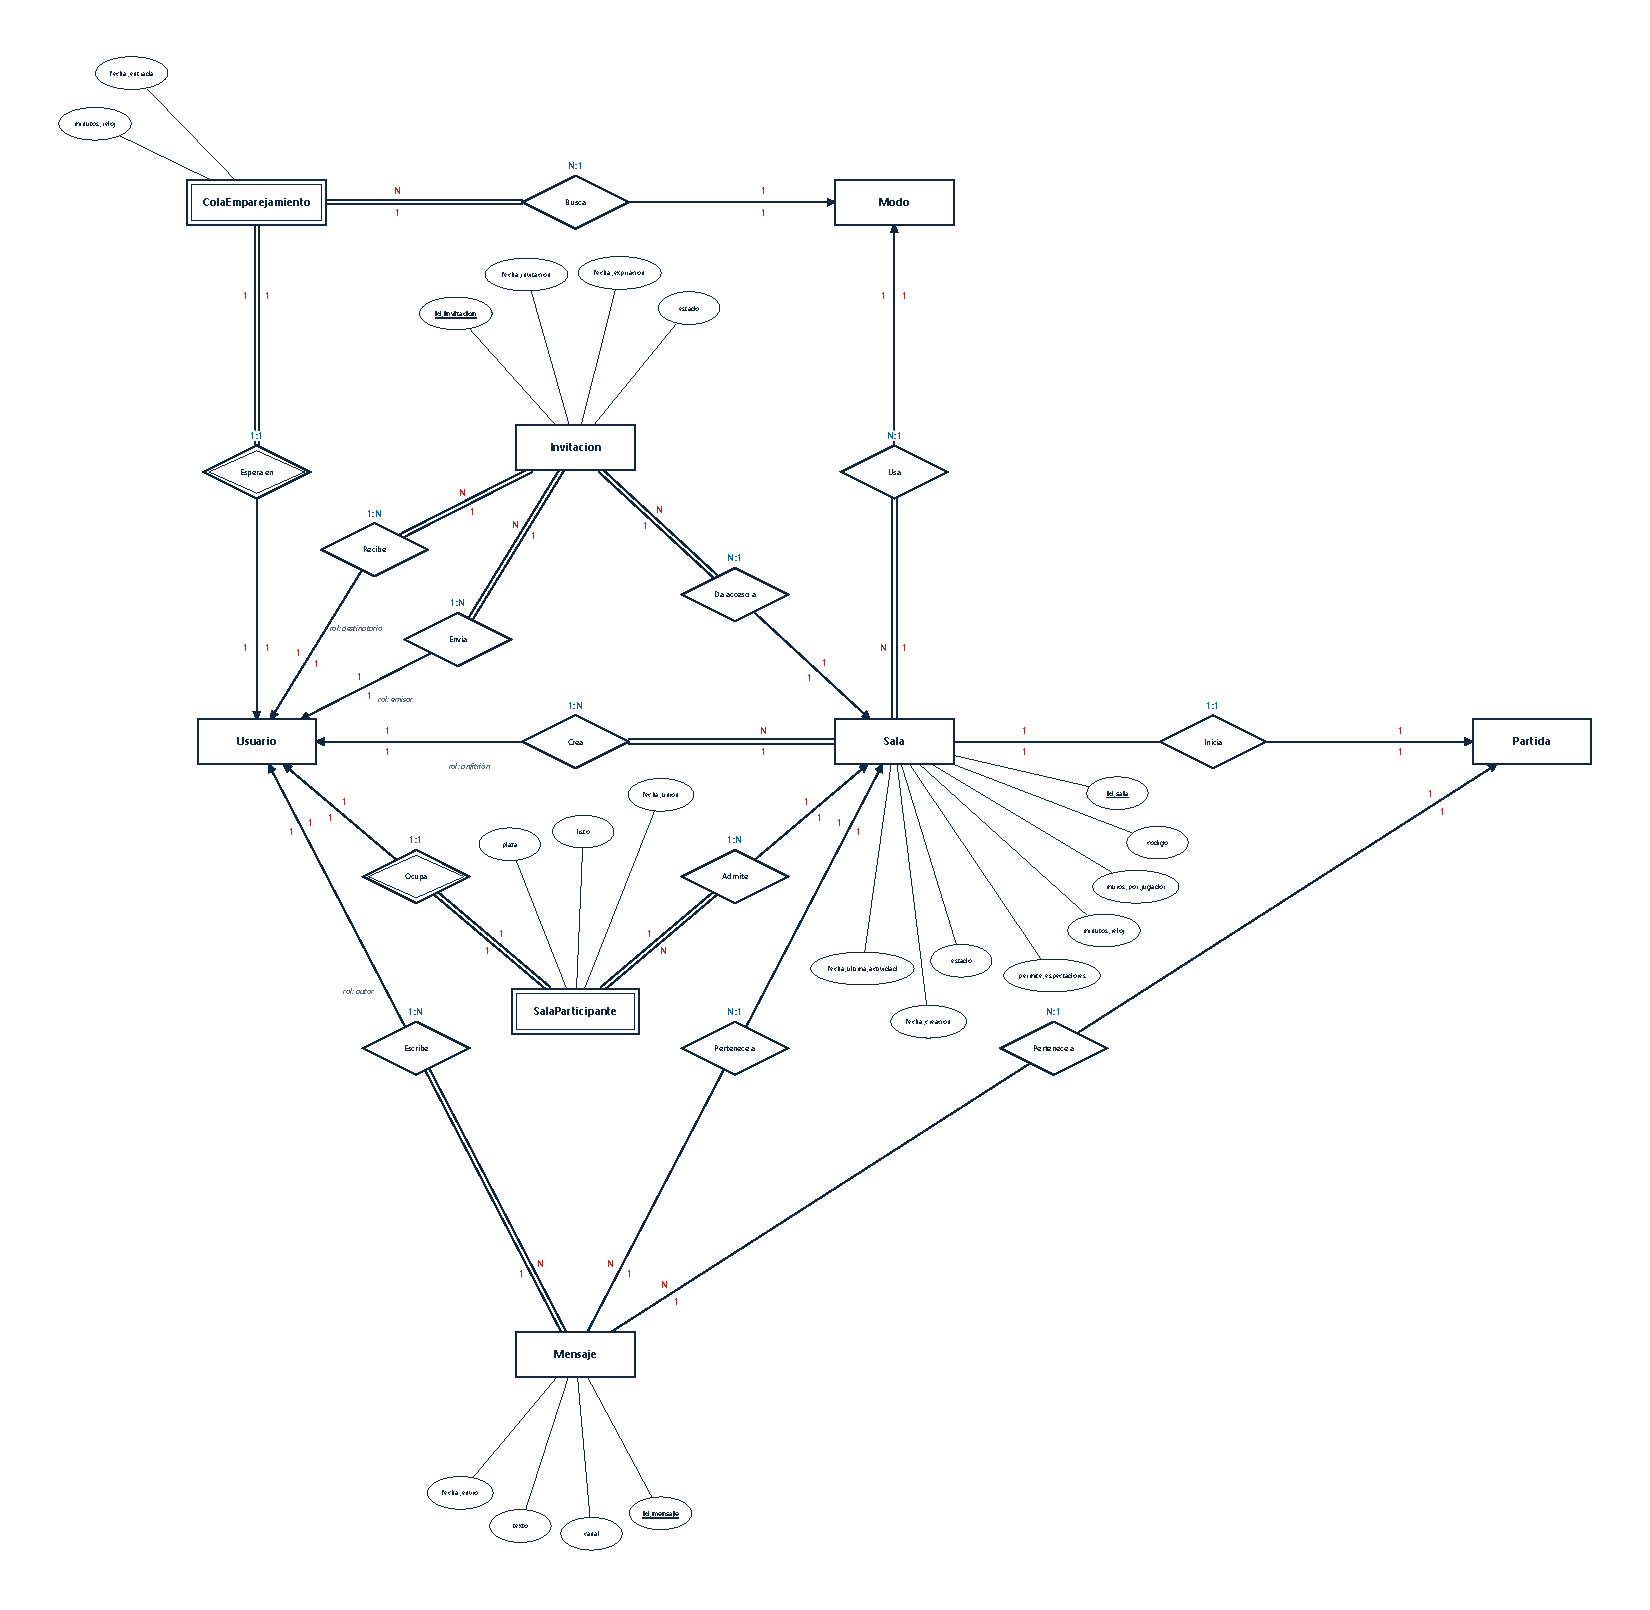
\includegraphics[width=\linewidth,height=0.82\textheight,keepaspectratio]{er/salida/salas}
\end{center}

\begin{landscape}
\subsubsection*{Clasificación y economía}
\addcontentsline{toc}{subsubsection}{Diagrama: clasificación y economía}
A la izquierda, las estadísticas por modo y los cambios de división; a la derecha, las cajas, su contenido y los movimientos de monedas.
\begin{center}
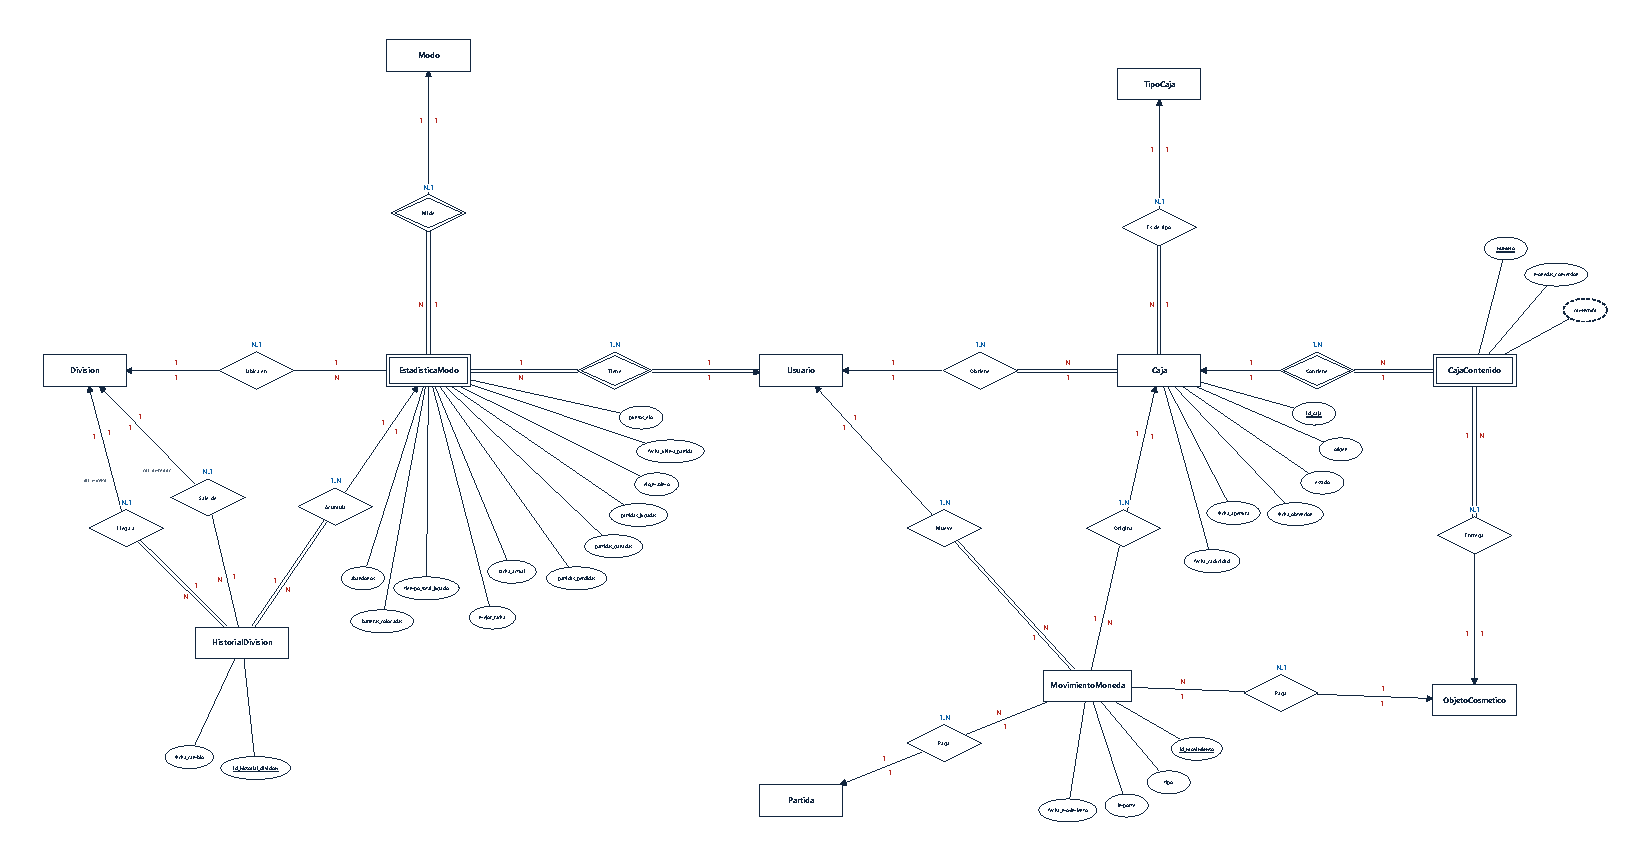
\includegraphics[width=\linewidth,height=0.8\textheight,keepaspectratio]{er/salida/economia}
\end{center}
\end{landscape}

\clearpage
\subsubsection*{Relaciones entre jugadores y tutorial}
\addcontentsline{toc}{subsubsection}{Diagrama: relaciones entre jugadores y tutorial}
Amistades, solicitudes, silencios y bloqueos, cada uno con dos relaciones hacia \textit{Usuario}, una por papel, y el avance de cada jugador en las lecciones del tutorial.
\begin{center}
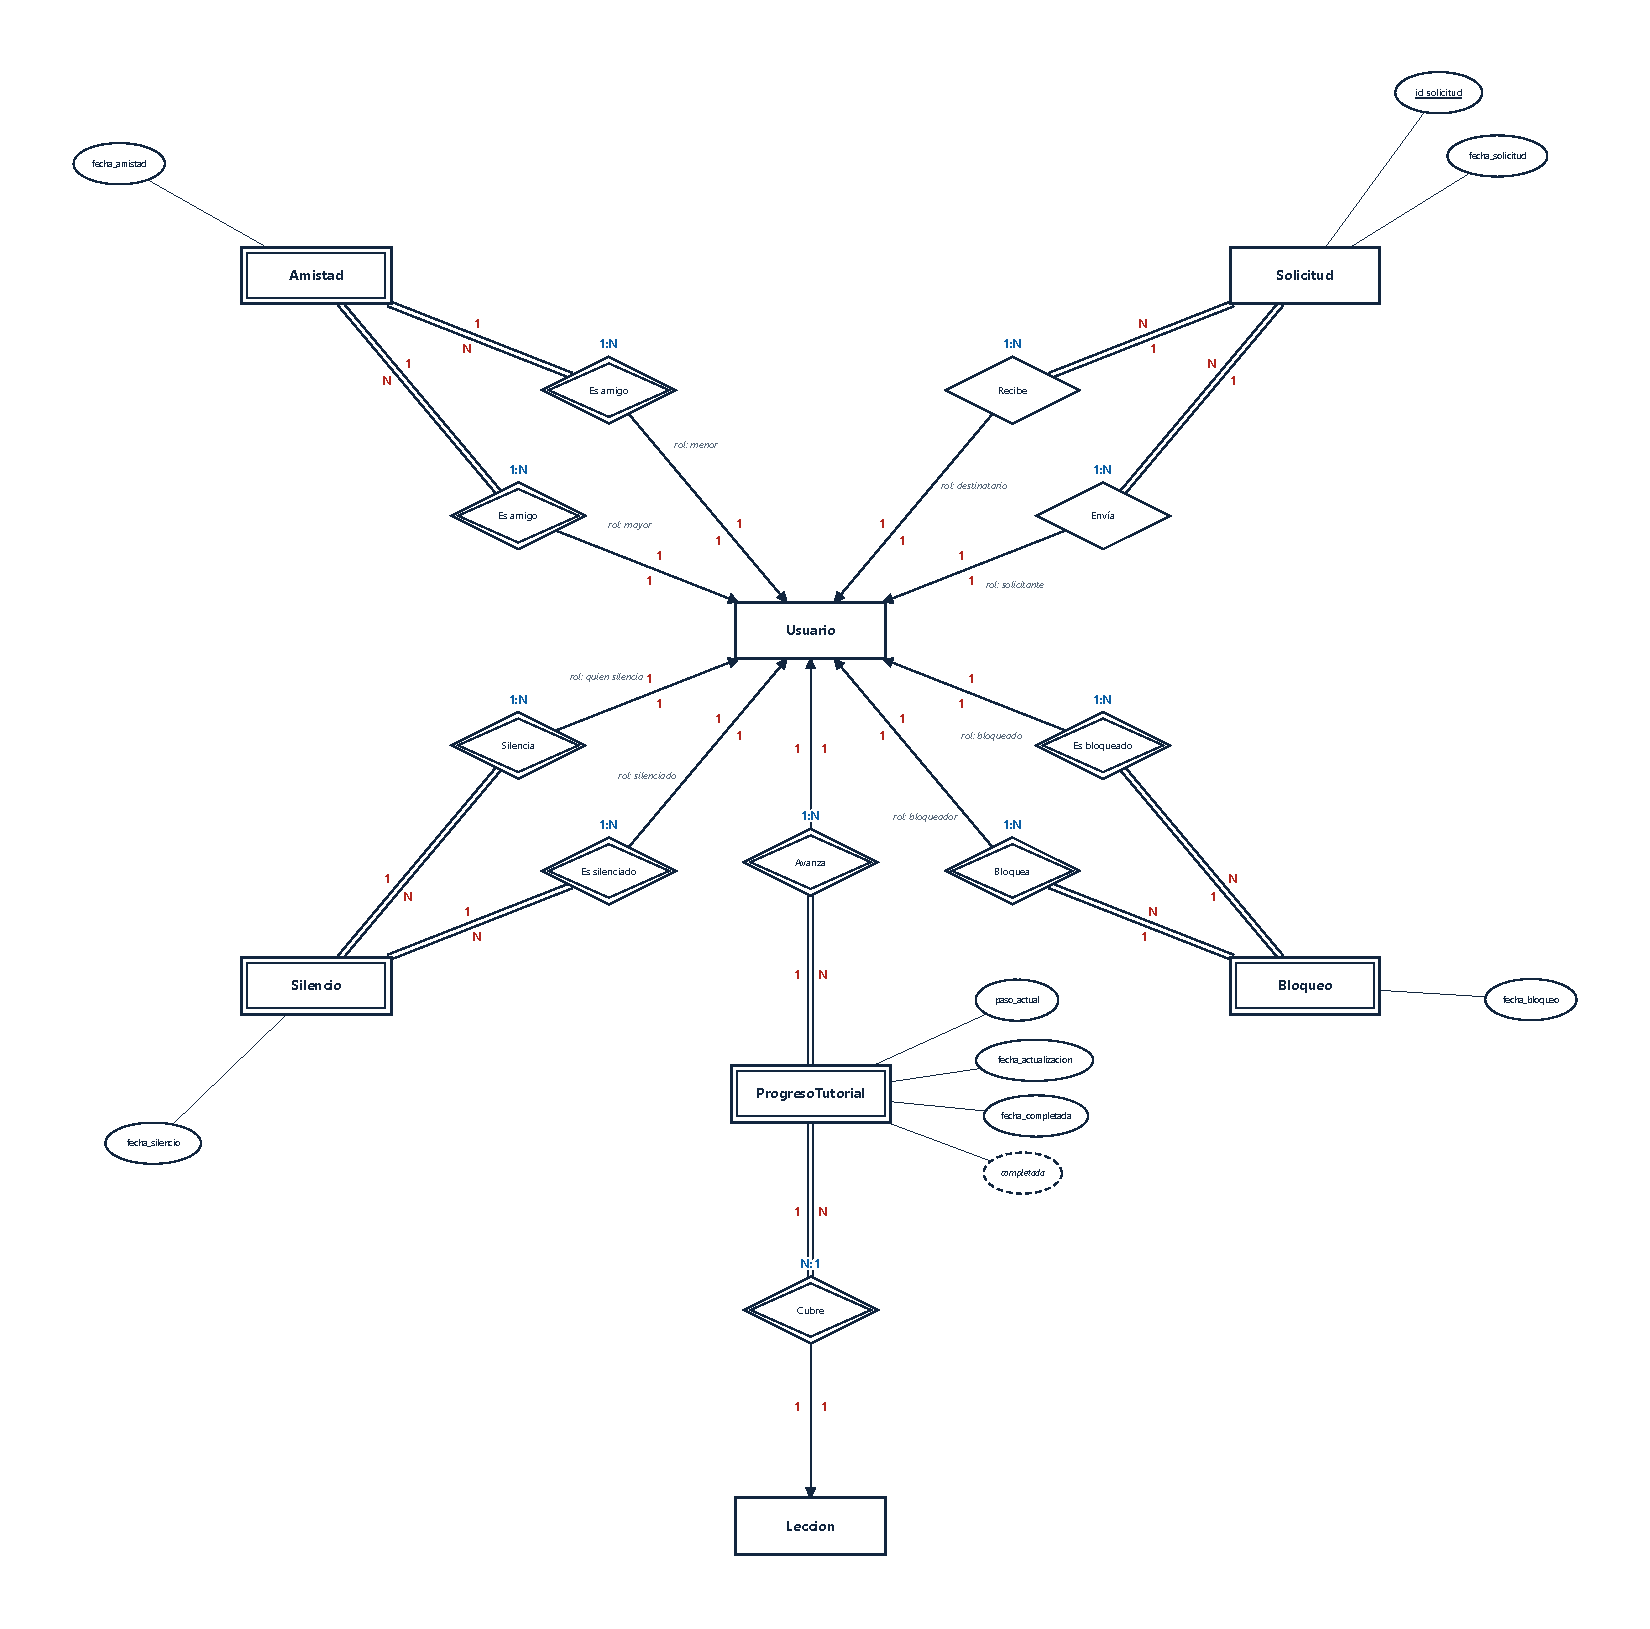
\includegraphics[width=\linewidth,height=0.82\textheight,keepaspectratio]{er/salida/social}
\end{center}

\clearpage
\subsubsection*{Moderación y bitácoras}
\addcontentsline{toc}{subsubsection}{Diagrama: moderación y bitácoras}
Reportes, sanciones, apelaciones y las dos bitácoras. El reporte se relaciona dos veces con \textit{Participacion} porque la partida adjunta tuvo que jugarla tanto el reportante como el reportado (\mbox{CU-42} \mbox{RN-09}).
\begin{center}
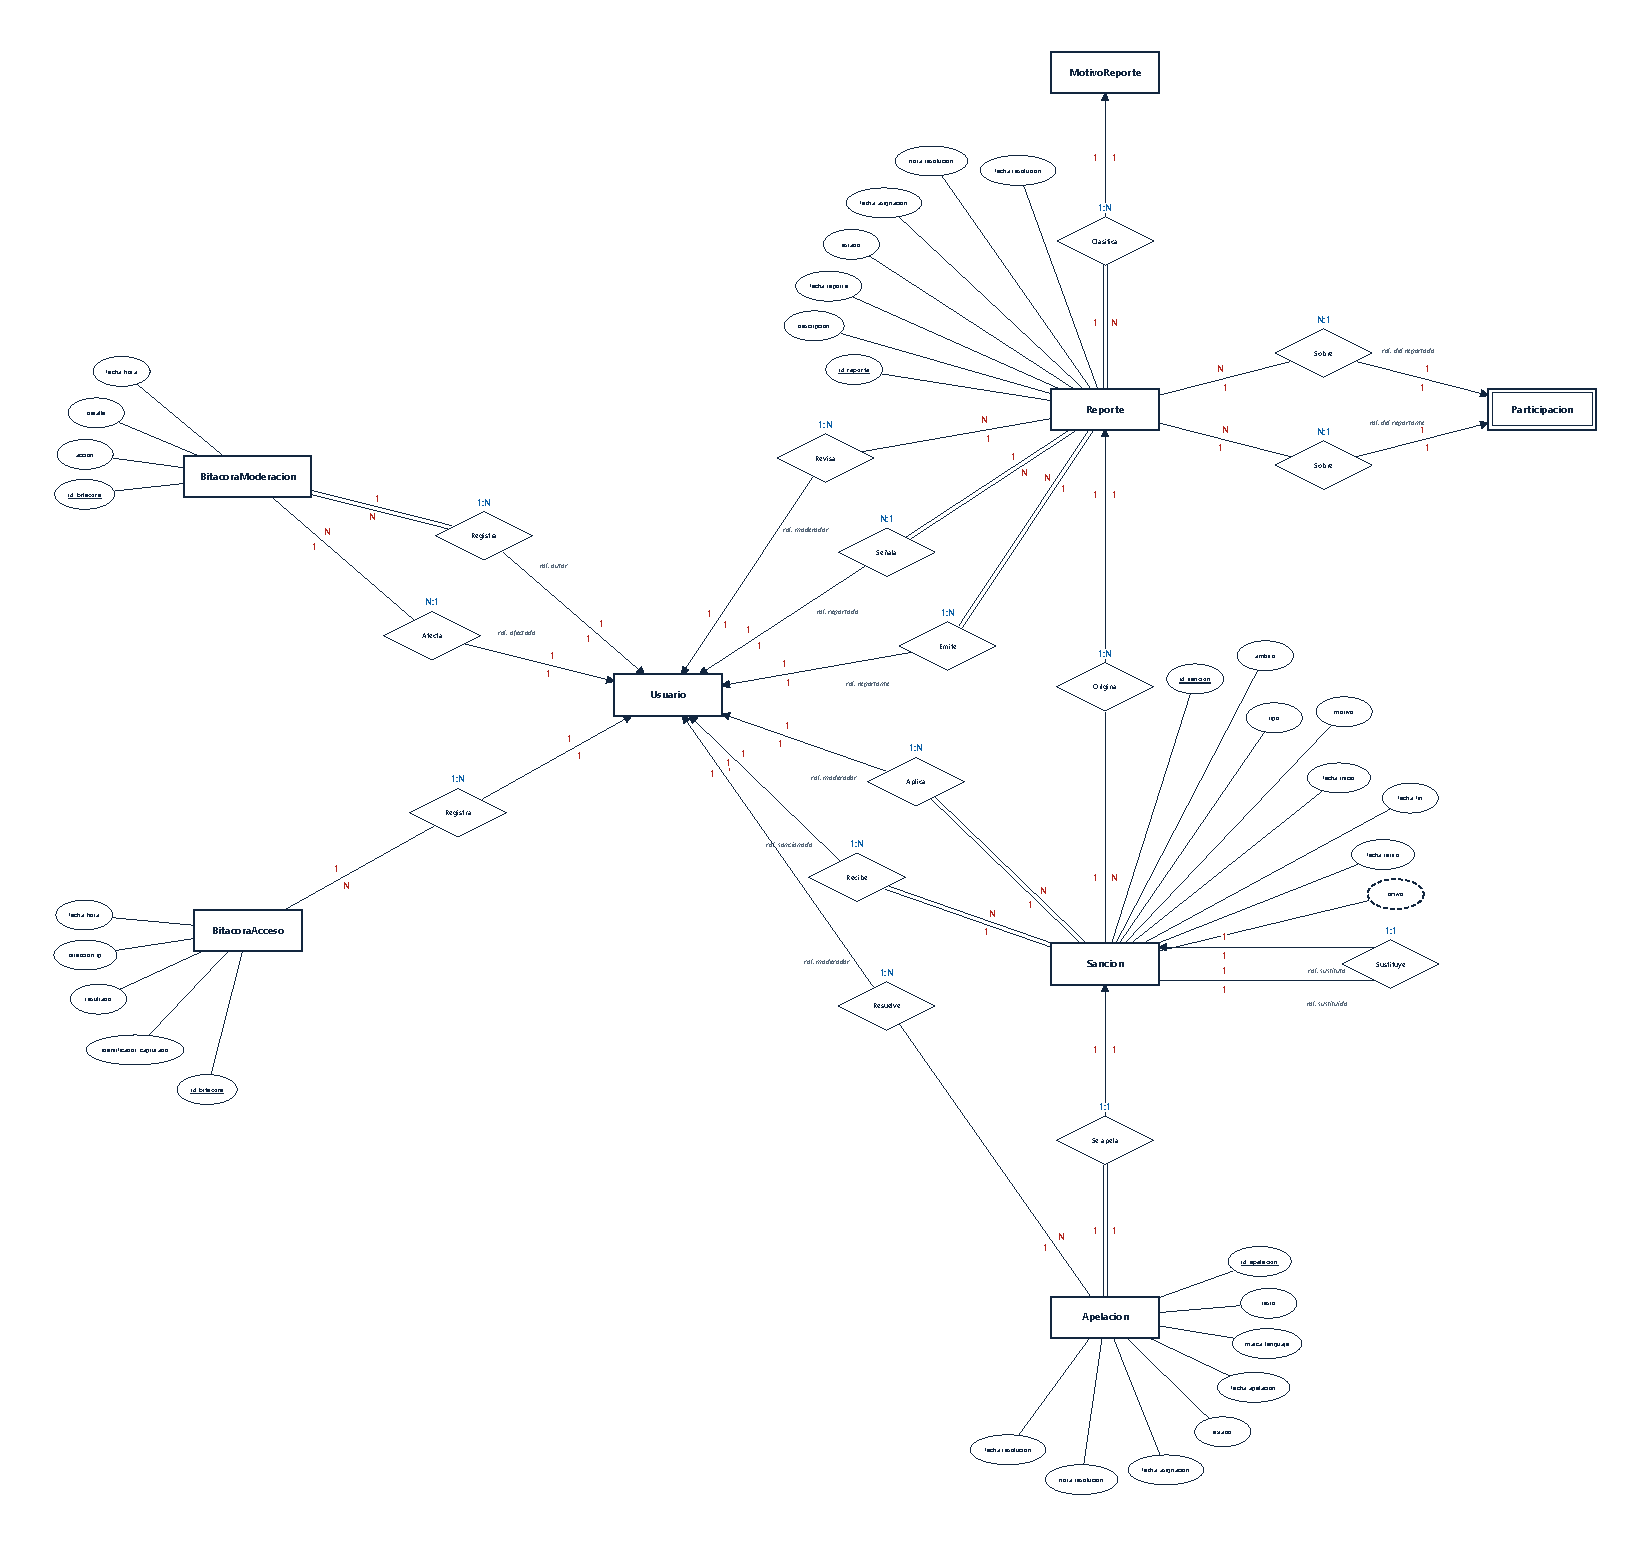
\includegraphics[width=\linewidth,height=0.82\textheight,keepaspectratio]{er/salida/moderacion}
\end{center}
\clearpage
